\documentclass[12pt,a4paper]{article}

% ── Packages ──────────────────────────────────────────────
\usepackage[margin=1in]{geometry}
\usepackage{pgfgantt}
\usepackage{amssymb}
\usepackage{tikz}
\usetikzlibrary{arrows.meta, positioning, shapes.geometric, calc}
\usepackage{booktabs}
\usepackage{longtable}
\usepackage{hyperref}
\usepackage{enumitem}
\usepackage{titlesec}
\usepackage{fancyhdr}
\usepackage{xcolor}
\usepackage{array}
\usepackage{graphicx}
\usepackage{tabularx}

% ── Colours ───────────────────────────────────────────────
\definecolor{phaseA}{HTML}{4A90D9}
\definecolor{phaseB}{HTML}{50C878}
\definecolor{phaseC}{HTML}{FF8C42}
\definecolor{phaseD}{HTML}{E8665D}
\definecolor{phaseE}{HTML}{9B59B6}
\definecolor{critical}{HTML}{E74C3C}
\definecolor{noncrit}{HTML}{3498DB}
\definecolor{headblue}{HTML}{1A5276}

% ── Section styling ───────────────────────────────────────
\titleformat{\section}
  {\Large\bfseries\color{headblue}}
  {\thesection.}{0.5em}{}[\vspace{2pt}\titlerule]
\titleformat{\subsection}
  {\large\bfseries\color{headblue!80}}
  {\thesubsection}{0.5em}{}

% ── Header / Footer ──────────────────────────────────────
\pagestyle{fancy}
\setlength{\headheight}{14.5pt}
\addtolength{\topmargin}{-2.5pt}
\fancyhf{}
\lhead{\small\textit{Software Project Plan --- Traffic Prediction System}}
\rhead{\small\textit{Group E-16}}
\cfoot{\thepage}

\begin{document}

% ═══════════════════════════════════════════════════════════
% TITLE PAGE
% ═══════════════════════════════════════════════════════════
\begin{titlepage}
\centering
\vspace*{2cm}
{\Huge\bfseries\color{headblue} Software Project Plan\\[12pt]}
{\LARGE Traffic Prediction and Analysis System\\[20pt]}
\rule{0.6\textwidth}{1pt}\\[20pt]

{\large\textbf{Assignment No. 7}}\\[30pt]

\begin{tabular}{ll}
\textbf{Group:} & E-16 \\[4pt]
\textbf{Members:} & Harshal Jaiswal \\
 & Pranav Jagtap \\
 & Suyash Jobanputra \\
 & Shreyash Jobanputra \\
\end{tabular}

\vfill
{\small Department of Computer Engineering\\
\today}
\end{titlepage}

% ═══════════════════════════════════════════════════════════
\section{Problem Statement}
% ═══════════════════════════════════════════════════════════
Prepare a detailed software project plan for the development of a \textbf{Traffic Prediction and Analysis System}. The project plan should incorporate scheduling techniques such as Gantt charts and PERT charts to map out the development timeline, visualize task dependencies, and determine the critical path of the project.

% ═══════════════════════════════════════════════════════════
\section{Abstract}
% ═══════════════════════════════════════════════════════════
Effective project planning forms the backbone of any successful software development endeavor. It encompasses task identification, effort estimation, dependency mapping, and continuous progress tracking. This document presents a comprehensive project plan for the \textbf{Traffic Prediction and Analysis System} --- a full-stack web application that leverages real-time data, historical patterns, and machine learning to forecast urban traffic congestion. The plan employs a Work Breakdown Structure (WBS), a Gantt chart for timeline visualization, and a PERT chart for dependency and critical path analysis, collectively providing a structured roadmap for the development lifecycle.

% ═══════════════════════════════════════════════════════════
\section{Introduction}
% ═══════════════════════════════════════════════════════════
Modern software systems demand rigorous planning to navigate the complexities of multi-module architectures, third-party integrations, and iterative feedback cycles. A well-defined project plan mitigates risks such as schedule overruns, scope creep, and inefficient resource allocation.

The \textbf{Traffic Prediction and Analysis System} addresses the challenge of urban traffic congestion by integrating data from Google Maps Directions API, OpenWeatherMap API, and Calendarific API with historical traffic records, construction and diversion updates, event schedules, and citizen-reported infrastructure defects. The system generates a weighted traffic score (0--100) for any given route and time slot, empowering commuters to make informed travel decisions.

Given the system's reliance on multiple data sources, a machine learning module (MobileNet for pothole detection), and a gamification engine for citizen engagement, meticulous scheduling across design, development, integration, and testing phases is essential.

\subsection{Planning Objectives}
The key objectives driving this project plan are:
\begin{enumerate}[noitemsep, label=\roman*)]
    \item Decompose the project into well-defined, manageable tasks.
    \item Estimate realistic durations for each development activity.
    \item Map inter-task dependencies to identify sequencing constraints.
    \item Construct a visual project schedule using industry-standard tools.
    \item Highlight the critical path to focus monitoring efforts.
    \item Anticipate risks and establish mitigation strategies.
\end{enumerate}

% ═══════════════════════════════════════════════════════════
\section{Development Phases}
% ═══════════════════════════════════════════════════════════
The project follows a phased software development approach. The lifecycle is divided into eight distinct phases, each contributing a critical deliverable:

\begin{center}
\begin{tabular}{cl}
\toprule
\textbf{\#} & \textbf{Phase} \\
\midrule
1 & Requirement Analysis \\
2 & System \& Architecture Design \\
3 & Database Schema Design \\
4 & Backend Development \\
5 & Frontend Development \\
6 & API \& ML Integration \\
7 & Testing \& Quality Assurance \\
8 & Deployment \& Documentation \\
\bottomrule
\end{tabular}
\end{center}

% ═══════════════════════════════════════════════════════════
\section{Work Breakdown Structure}
% ═══════════════════════════════════════════════════════════
The WBS decomposes the project into discrete tasks with estimated durations and explicit dependency chains.

\bigskip
\begin{center}
\begin{tabular}{c l c l}
\toprule
\textbf{ID} & \textbf{Task} & \textbf{Duration} & \textbf{Depends On} \\
\midrule
T1 & Requirement Analysis & 2 Weeks & --- \\
T2 & System \& Architecture Design & 2 Weeks & T1 \\
T3 & Database Schema Design & 2 Weeks & T1 \\
T4 & Backend Development & 4 Weeks & T2, T3 \\
T5 & Frontend Development & 3 Weeks & T2, T3 \\
T6 & API \& ML Integration & 3 Weeks & T4, T5 \\
T7 & Testing \& Quality Assurance & 2 Weeks & T6 \\
T8 & Deployment \& Documentation & 2 Weeks & T7 \\
\bottomrule
\end{tabular}
\end{center}

\subsection{Task Descriptions}

\textbf{T1 --- Requirement Analysis (2 Weeks):}
Involves stakeholder interviews, feature prioritization, and preparation of the IEEE 830 SRS document. Core requirements include traffic prediction, pothole reporting with ML verification, citizen gamification, and an admin dashboard.

\textbf{T2 --- System \& Architecture Design (2 Weeks):}
Defines the MVC architecture pattern using Node.js/Express for the backend and React.js for the frontend. Includes API endpoint specification, service layer design, and interaction diagrams for the prediction engine and external API modules.

\textbf{T3 --- Database Schema Design (2 Weeks):}
Creates 19+ MongoDB collections covering Users, PathInfo (traffic scores), Complaints, Images (potholes), Events, Construction zones, Diversions, Schools, Hospitals, Hotels, Malls, HotspotLocations, PredictionLogs, and TrafficStatus records.

\textbf{T4 --- Backend Development (4 Weeks):}
Implements JWT-based authentication, the weighted traffic prediction engine (7 factors: Historical 25\%, Weather 15\%, Construction 15\%, Events 20\%, Hotspots 12\%, Potholes 8\%, Complaints 5\%), the automated cron-based data collector, gamification scoring, and 22 REST API controllers.

\textbf{T5 --- Frontend Development (3 Weeks):}
Builds the React.js single-page application with interactive traffic maps (Google Maps integration), prediction result cards, pothole image upload with camera capture, citizen score leaderboard, and the admin management dashboard.

\textbf{T6 --- API \& ML Integration (3 Weeks):}
Connects frontend to backend APIs. Integrates Google Maps Directions, OpenWeatherMap, and Calendarific external services. Deploys the MobileNet pothole detection model and configures Cloudinary for image storage.

\textbf{T7 --- Testing \& Quality Assurance (2 Weeks):}
Unit tests for individual modules, integration tests for API-to-database flows, and User Acceptance Testing (UAT) with performance benchmarking of the prediction engine under concurrent load.

\textbf{T8 --- Deployment \& Documentation (2 Weeks):}
Production deployment on Render (backend) and Vercel (frontend). Finalizes blackbook documentation, user guide, and project handover materials.

% ═══════════════════════════════════════════════════════════
\section{Project Scheduling}
% ═══════════════════════════════════════════════════════════

\subsection{Gantt Chart}
The Gantt chart below maps each task against a 20-week timeline, with color-coded bars indicating the project phase and arrows denoting task dependencies.

\bigskip
\begin{center}
\resizebox{\textwidth}{!}{%
\begin{ganttchart}[
    hgrid,
    vgrid={*{3}{draw=gray!30}, *1{draw=gray!60}},
    x unit=0.6cm,
    y unit chart=0.7cm,
    title height=1,
    title label font=\small\bfseries,
    bar label font=\small,
    bar height=0.6,
    group/.append style={fill=black!80},
    group label font=\small\bfseries,
    link/.style={->, thick}
]{1}{20}

  \gantttitle{Project Timeline (Weeks)}{20} \\
  \gantttitlelist{1,...,20}{1} \\

  \ganttbar[bar/.append style={fill=phaseA}, name=t1]{T1: Requirement Analysis}{1}{2} \\
  \ganttbar[bar/.append style={fill=phaseA}, name=t2]{T2: System Design}{3}{4} \\
  \ganttbar[bar/.append style={fill=phaseB}, name=t3]{T3: Database Design}{3}{4} \\
  \ganttbar[bar/.append style={fill=phaseC}, name=t4]{T4: Backend Development}{5}{8} \\
  \ganttbar[bar/.append style={fill=phaseC}, name=t5]{T5: Frontend Development}{6}{8} \\
  \ganttbar[bar/.append style={fill=phaseC}, name=t6]{T6: API \& ML Integration}{9}{11} \\
  \ganttbar[bar/.append style={fill=phaseD}, name=t7]{T7: Testing \& QA}{12}{13} \\
  \ganttbar[bar/.append style={fill=phaseE}, name=t8]{T8: Deployment \& Docs}{14}{15} \\

  \ganttlink{t1}{t2}
  \ganttlink{t1}{t3}
  \ganttlink{t2}{t4}
  \ganttlink{t3}{t4}
  \ganttlink{t2}{t5}
  \ganttlink{t4}{t6}
  \ganttlink{t5}{t6}
  \ganttlink{t6}{t7}
  \ganttlink{t7}{t8}

\end{ganttchart}
}% end resizebox
\end{center}

\medskip
\noindent\textbf{Legend:}
\textcolor{phaseA}{$\blacksquare$}~Planning \quad
\textcolor{phaseB}{$\blacksquare$}~Database \quad
\textcolor{phaseC}{$\blacksquare$}~Development \quad
\textcolor{phaseD}{$\blacksquare$}~Testing \quad
\textcolor{phaseE}{$\blacksquare$}~Deployment

\begin{center}
\small\textit{Figure 1: Gantt Chart --- Traffic Prediction and Analysis System}
\end{center}

\subsection{Gantt Chart Analysis}
The timeline reveals that T2 (System Design) and T3 (Database Design) execute \textbf{concurrently} after T1, reducing the schedule by 2 weeks compared to sequential execution. Backend (T4) and Frontend (T5) development also overlap during weeks 6--8, enabling parallel workstreams across the team. The integration phase (T6) acts as a synchronization point, beginning only after both T4 and T5 are complete. The total planned duration spans \textbf{15 active weeks} with 5 weeks of buffer within the 20-week window.

% ═══════════════════════════════════════════════════════════
\subsection{PERT Chart}
The PERT diagram represents tasks as nodes with directed edges indicating dependencies. The \textcolor{critical}{\textbf{critical path}} is highlighted in red.

\bigskip
\begin{center}
\resizebox{\textwidth}{!}{%
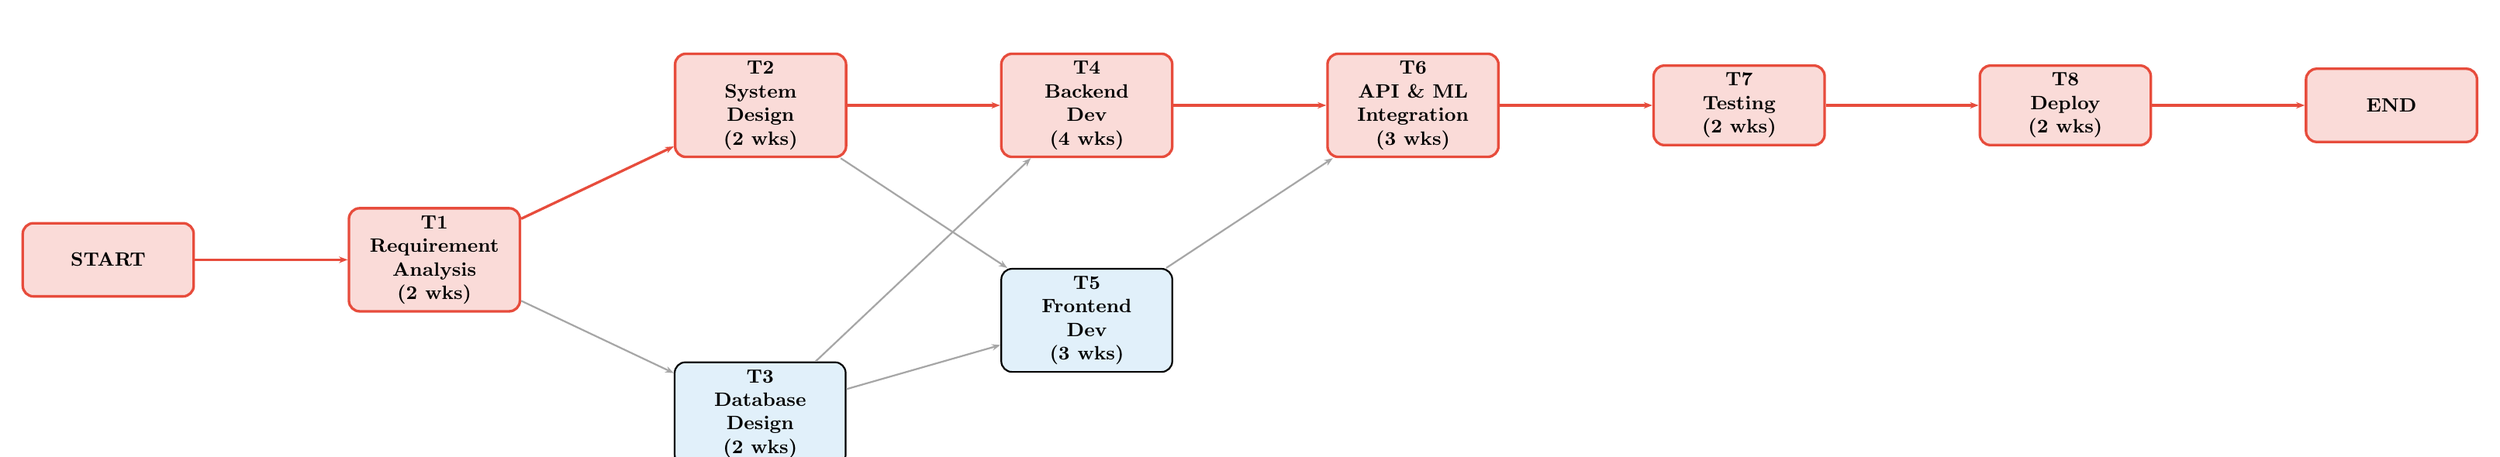
\begin{tikzpicture}[
    node distance=1.8cm and 2.5cm,
    task/.style={
        rectangle, rounded corners=5pt, draw, thick,
        minimum width=2.8cm, minimum height=1.2cm,
        align=center, font=\small\bfseries,
        fill=noncrit!15, text=black
    },
    crit/.style={
        task, fill=critical!20, draw=critical, very thick
    },
    arr/.style={-{Stealth[length=4pt]}, thick, gray!70},
    critarr/.style={-{Stealth[length=4pt]}, very thick, critical},
]

\node[crit] (start) {START};
\node[crit, right=of start] (T1) {T1\\Requirement\\Analysis\\(2 wks)};
\node[crit, above right=0.8cm and 2.5cm of T1] (T2) {T2\\System\\Design\\(2 wks)};
\node[task, below right=0.8cm and 2.5cm of T1] (T3) {T3\\Database\\Design\\(2 wks)};
\node[crit, right=of T2] (T4) {T4\\Backend\\Dev\\(4 wks)};
\node[task, below=1.8cm of T4] (T5) {T5\\Frontend\\Dev\\(3 wks)};
\node[crit, right=of T4] (T6) {T6\\API \& ML\\Integration\\(3 wks)};
\node[crit, right=of T6] (T7) {T7\\Testing\\(2 wks)};
\node[crit, right=of T7] (T8) {T8\\Deploy\\(2 wks)};
\node[crit, right=of T8] (finish) {END};

% ── Critical Path (Red) ──────
\draw[critarr] (start) -- (T1);
\draw[critarr] (T1) -- (T2);
\draw[critarr] (T2) -- (T4);
\draw[critarr] (T4) -- (T6);
\draw[critarr] (T6) -- (T7);
\draw[critarr] (T7) -- (T8);
\draw[critarr] (T8) -- (finish);

% ── Non-Critical (Gray) ──────
\draw[arr] (T1) -- (T3);
\draw[arr] (T3) -- (T4);
\draw[arr] (T2) -- (T5);
\draw[arr] (T3) -- (T5);
\draw[arr] (T5) -- (T6);

\end{tikzpicture}
}% end resizebox
\end{center}

\begin{center}
\small\textit{Figure 2: PERT Chart --- Task Dependencies and Critical Path}
\end{center}

\subsection{Critical Path Identification}
The critical path comprises the longest chain of dependent tasks:

\begin{center}
\textcolor{critical}{\textbf{T1 $\rightarrow$ T2 $\rightarrow$ T4 $\rightarrow$ T6 $\rightarrow$ T7 $\rightarrow$ T8}}
\end{center}

\begin{center}
\begin{tabular}{lcc}
\toprule
\textbf{Task} & \textbf{Duration} & \textbf{Cumulative} \\
\midrule
T1: Requirement Analysis & 2 wks & 2 wks \\
T2: System Design & 2 wks & 4 wks \\
T4: Backend Development & 4 wks & 8 wks \\
T6: API \& ML Integration & 3 wks & 11 wks \\
T7: Testing \& QA & 2 wks & 13 wks \\
T8: Deployment & 2 wks & \textbf{15 wks} \\
\bottomrule
\end{tabular}
\end{center}

\noindent Any delay in a critical-path task directly extends the project deadline. Non-critical tasks T3 (Database Design), and T5 (Frontend Development) carry \textbf{2--3 weeks of float}, meaning minor delays in these tasks will not impact the overall schedule.

% ═══════════════════════════════════════════════════════════
\section{Risk Assessment}
% ═══════════════════════════════════════════════════════════

\begin{center}
\begin{tabularx}{\textwidth}{l X l}
\toprule
\textbf{Risk} & \textbf{Description} & \textbf{Mitigation} \\
\midrule
API Limits & Google Maps / OpenWeatherMap impose daily rate caps & 15-min response caching \\[4pt]
ML Accuracy & MobileNet pothole detection may produce false positives & Confidence threshold $\geq 0.85$ + admin review \\[4pt]
Data Gaps & Limited historical traffic data for newly added routes & Backfill scripts + city-average fallback \\[4pt]
Integration & Frontend--Backend API contract mismatches & Shared API specification document \\[4pt]
Performance & Slow response under concurrent predictions & Database indexing + query optimization \\[4pt]
Availability & Team bandwidth reduced during exams & 5-week slack in non-critical tasks \\
\bottomrule
\end{tabularx}
\end{center}

% ═══════════════════════════════════════════════════════════
\section{Conclusion}
% ═══════════════════════════════════════════════════════════
This document presented a structured project plan for the Traffic Prediction and Analysis System. The Work Breakdown Structure decomposed the project into eight manageable tasks, the Gantt chart provided a visual timeline with concurrent workstreams, and the PERT chart identified a 15-week critical path through the project lifecycle.

By leveraging these industry-standard project management techniques, the development team can systematically track progress, allocate resources efficiently, and deliver the system within the planned schedule while maintaining quality standards.

\end{document}
